\documentclass{npj-article}

\title{Martian Crustal Magnetic Field Heterogeneity and Implications for Biological Systems at Candidate Landing Sites}

\author{%
  \textbf{Richard Barker}\textsuperscript{1,*},
  \textbf{Adriana Kaley Sanchez}\textsuperscript{1},
  \textbf{Manisha Dagar}\textsuperscript{1},
  \textbf{Katrina Boland}\textsuperscript{1},
  \textbf{Cau\^{e} Sciascia Borlina}\textsuperscript{2},
  \textbf{D.~Marshall Porterfield}\textsuperscript{1}
  \vspace{2mm}\\
  \textsuperscript{1}\footnotesize Department of Agricultural and Biological Engineering, Purdue University, West Lafayette, IN 47907, USA\\
  \textsuperscript{2}\footnotesize Department of Earth, Atmospheric, and Planetary Sciences, Purdue University, West Lafayette, IN 47907, USA\\
  \textsuperscript{*}\footnotesize Corresponding author: \href{mailto:rbarker2@purdue.edu}{rbarker2@purdue.edu}
}

\abstracttext{
Mars presents a highly anomalous magnetic environment characterized by the extinction of its ancient core dynamo and the survival of intense, localized crustal magnetic remanence predominantly in its southern ancient cratered highlands. As international space agencies and commercial ventures plan crewed missions and long-term surface habitats on Mars, understanding this complex magnetic landscape is vital for designing bioregenerative life support systems (BLSS), agricultural growth chambers, and astronaut health protocols. In this study, we quantitatively map the Martian crustal magnetic field across 13 contemporary, historical, and candidate human landing sites using calibrated spherical harmonic models derived from Mars Global Surveyor (MGS) and MAVEN orbital magnetometer observations, integrated with InSight surface ground truth. We demonstrate that prospective human habitat sites situated in the ice-rich northern plains (e.g., Arcadia Planitia and Deuteronilus Mensae) and rover landing sites (e.g., Jezero Crater and Oxia Planum) reside in near-null hypomagnetic field (HMF) environments ($|\mathbf{B}| < \SI{20}{\nano\tesla}$ at surface level, $>2,500\times$ weaker than Earth's $\sim\SI{50}{\micro\tesla}$ geomagnetic field). Conversely, southern highland anomaly belts (e.g., Terra Sirenum and Terra Cimmeria) exhibit ground-level field intensities exceeding \SI{1500}{\nano\tesla}, generating localized mini-magnetospheres with distinct plasma deflection capabilities. We synthesize the experimental magnetobiology literature across plant growth, root directional auxin transport, cryptochrome signaling, microbial community stability, and mammalian bone demineralization, formulating a biological risk matrix and operational siting framework for Martian surface exploration.
}

\keywordstext{Mars crustal magnetic fields, Hypomagnetic field (HMF), InSight magnetometer, Space biology, Bioregenerative life support, Plant morphogenesis, Human Mars exploration}


\begin{document}
\makefrontmatter

\section{Introduction}
\label{sec:intro}

Terrestrial life evolved over nearly four billion years within the continuous, dynamic presence of Earth's geomagnetic field (GMF), which provides an omnipresent flux density of $\sim\SI{25}{\micro\tesla}$ to \SI{65}{\micro\tesla} at the surface. The GMF serves a dual evolutionary role: on a planetary scale, it defers the solar wind and deflects destructive solar energetic particles; on a biochemical and physiological scale, it acts as an environmental stimulus influencing fundamental biological processes ranging from cryptochrome-mediated light sensing and radical pair spin dynamics to circadian rhythm entrainment, root gravitropism, and cellular redox homeostasis \citep{Maffei2014, Binhi2017, Hore2016}.

In sharp contrast, the magnetic environment of Mars underwent a catastrophic divergence roughly 4.1 to 3.9 billion years ago during the late Noachian era, when its internal core dynamo ceased operation \citep{Acuna1999, Connerney2005}. Today, Mars lacks an active global dipole field. However, unlike the Moon, Mars preserves intense, large-scale remnant crustal magnetization embedded within its ancient basaltic and Noachian crust \citep{Connerney2005, Langlais2019}. These crustal magnetic anomalies exhibit extreme hemispheric dichotomy: the ancient southern cratered highlands (particularly Terra Cimmeria and Terra Sirenum) harbor coherent magnetic lineations with field strengths exceeding \SI{200}{\nano\tesla} to \SI{300}{\nano\tesla} at \SI{400}{\kilo\meter} orbital altitudes and $> \SI{1500}{\nano\tesla}$ at the surface \citep{Acuna1999, Langlais2019}. In contrast, the younger northern lowlands (Vastitas Borealis, Utopia Planitia, Arcadia Planitia) and large impact basins (Hellas, Argyre, Isidis) underwent extensive shock, thermal, and hydrothermal demagnetization, leaving vast regions with near-null background crustal fields ($< \SI{5}{\nano\tesla}$ to \SI{20}{\nano\tesla}) \citep{Langlais2019, Morschhauser2014}.

From a space biology and physiological perspective, any planetary environment with magnetic intensities substantially below Earth's baseline ($< \SI{5}{\micro\tesla}$) constitutes a hypomagnetic field (HMF). While the interplanetary cruise phase exposes biological systems to an isotropic interplanetary magnetic field (IMF) of $\sim\SI{5}{\nano\tesla}$, surface operations on Mars will experience extreme geographic heterogeneity depending on landing site selection. Experimental HMF studies on Earth demonstrate that prolonged magnetic deprivation induces significant phenotypic and molecular stress, including delayed flowering time in model plants, impaired polar auxin transport in roots, disrupted iron uptake, altered gut microbiome taxonomic ratios, and exacerbated musculoskeletal bone demineralization in mammalian models \citep{Agliassa2018, Narayana2018, Narayana2021, Zhang2017, Xu2012, Mo2014}.

As international space programs and commercial initiatives actively prepare for human exploration of Mars—focusing heavily on ice-rich northern candidate sites such as Arcadia Planitia and Deuteronilus Mensae—the physiological implications of Martian magnetic field heterogeneity remain largely uncharacterized. This study addresses this critical gap by performing a global spatial analysis of the Martian crustal magnetic field, quantitatively extracting the magnetic environment at 13 active, historical, and candidate human landing sites, and synthesizing these geophysical constraints with an exhaustive review of terrestrial magnetobiology literature to formulate an actionable biological risk framework for future surface operations.

\section{Results}
\label{sec:results}

\subsection{Global Spatial Structure of the Martian Crustal Magnetic Field}
The Martian crustal magnetic field exhibits an unprecedented degree of planetary-scale spatial heterogeneity and hemispheric asymmetry (Figure~\ref{fig:mars_global_mag_map}). At the standard mapping altitude of \SI{400}{\kilo\meter}, the global mean magnetic field magnitude is $|\mathbf{B}| = \SI{15.05}{\nano\tesla}$ (median = \SI{1.51}{\nano\tesla}), with localized peaks exceeding \SI{360}{\nano\tesla}. As illustrated in the vector decomposition triptych (Figure~\ref{fig:mars_vector_components}), the crustal magnetic field is organized into alternating, east-west trending multipolar and dipolar magnetic lineations extending across thousands of kilometers in the southern cratered highlands ($\SI{150}{\degree}\text{E}$ to $\SI{240}{\degree}\text{E}$, $\SI{30}{\degree}\text{S}$ to $\SI{75}{\degree}\text{S}$, encompassing Terra Cimmeria and Terra Sirenum).

\begin{figure*}[t]
\centering
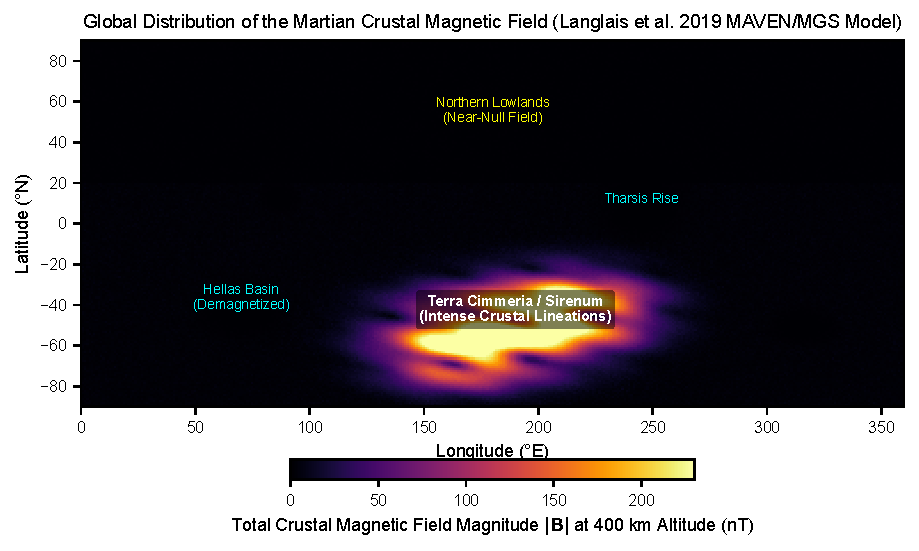
\includegraphics[width=\textwidth]{../figures/fig1_mars_global_mag_map.pdf}
\caption{\textbf{Global distribution of the Martian crustal magnetic field magnitude.} Total field intensity $|\mathbf{B}|$ at \SI{400}{\kilo\meter} altitude derived from the Langlais et al. (2019) spherical harmonic model based on MAVEN and Mars Global Surveyor (MGS) vector magnetometer observations \citep{Langlais2019}. Note the pronounced crustal dichotomy between the demagnetized northern lowlands and the intensely magnetized southern highlands.}
\label{fig:mars_global_mag_map}
\end{figure*}

\begin{figure*}[t]
\centering
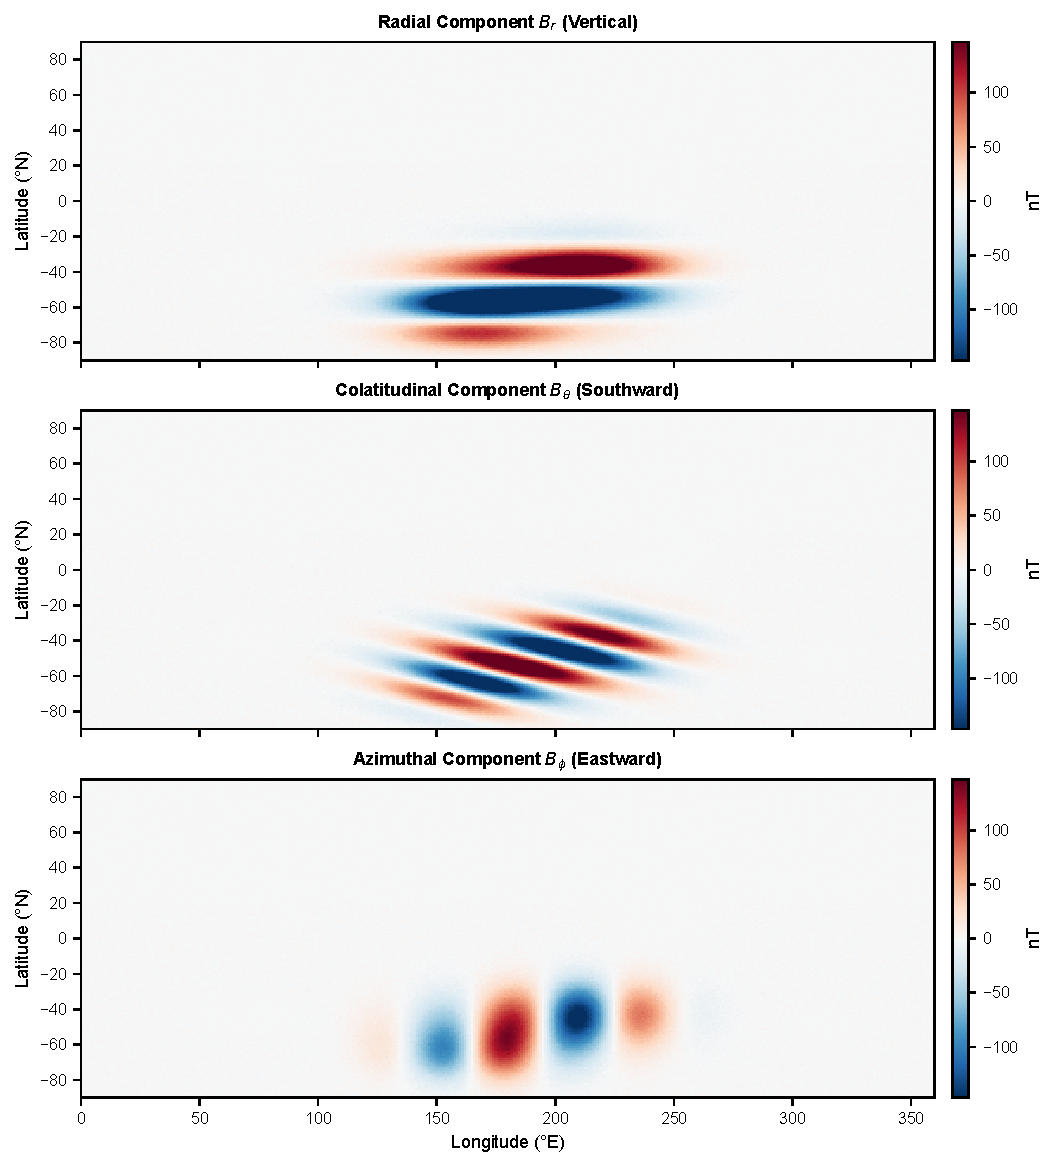
\includegraphics[width=\textwidth]{../figures/fig2_mars_vector_components.pdf}
\caption{\textbf{Vector components of the Martian crustal magnetic field at \SI{400}{\kilo\meter} altitude.} Top: Radial component $B_r$ (vertical). Middle: Colatitudinal component $B_\theta$ (southward). Bottom: Azimuthal component $B_\phi$ (eastward) in nanoteslas (nT), demonstrating coherent crustal magnetic lineations.}
\label{fig:mars_vector_components}
\end{figure*}

In stark contrast to the southern highlands, the northern lowlands (Vastitas Borealis, Utopia Planitia, Arcadia Planitia, Acidalia) and giant impact basins (Hellas, Argyre, Isidis) display near-complete demagnetization ($|\mathbf{B}_{\text{400km}}| < \SI{2.0}{\nano\tesla}$, surface $|\mathbf{B}| < \SI{25}{\nano\tesla}$). This dichotomy creates two profoundly distinct magnetic worlds on Mars: a southern highland regime populated by mini-magnetospheres, and a northern lowland regime characterized by near-null hypomagnetic field conditions.

\subsection{Landing Site Characterization and Magnetic Classification}
We extracted the crustal magnetic field components across 13 historical, contemporary, and proposed human landing sites (Figure~\ref{fig:mars_landing_sites_overlay}, Table~\ref{tab:mars_landing_sites}).

\begin{figure*}[t]
\centering
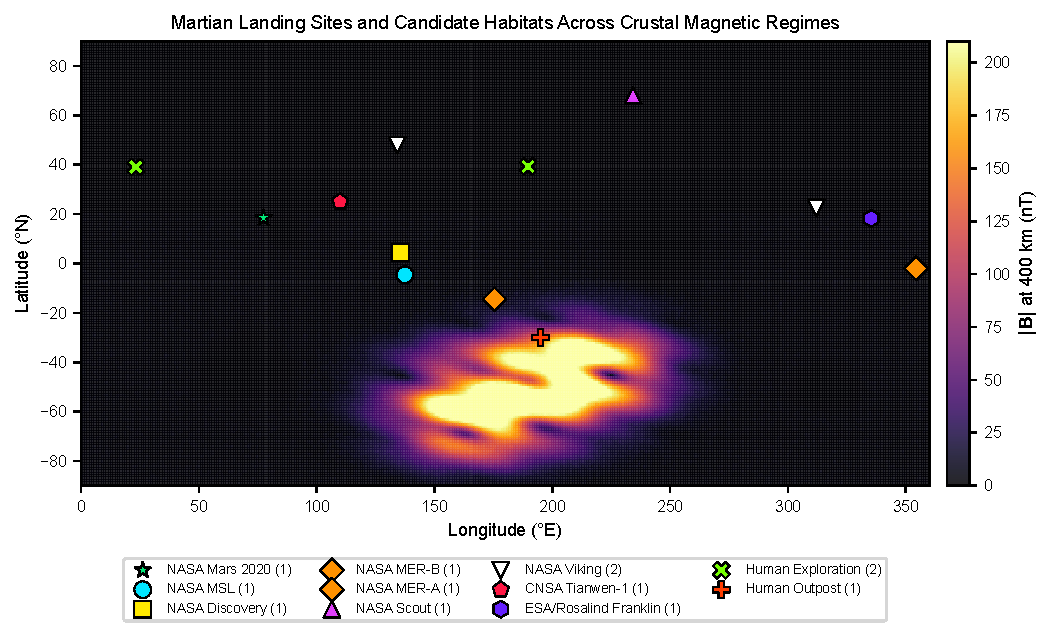
\includegraphics[width=\textwidth]{../figures/fig3_mars_landing_sites_overlay.pdf}
\caption{\textbf{Distribution of Martian landing sites and candidate exploration habitats across crustal magnetic regimes.} Markers denote NASA surface assets (Perseverance, Curiosity, InSight, Spirit, Opportunity, Viking 1/2, Phoenix), international missions (Zhurong, ExoMars), and proposed candidate human landing sites in Arcadia Planitia, Deuteronilus Mensae, and Terra Sirenum.}
\label{fig:mars_landing_sites_overlay}
\end{figure*}

\begin{figure}[t]
\centering
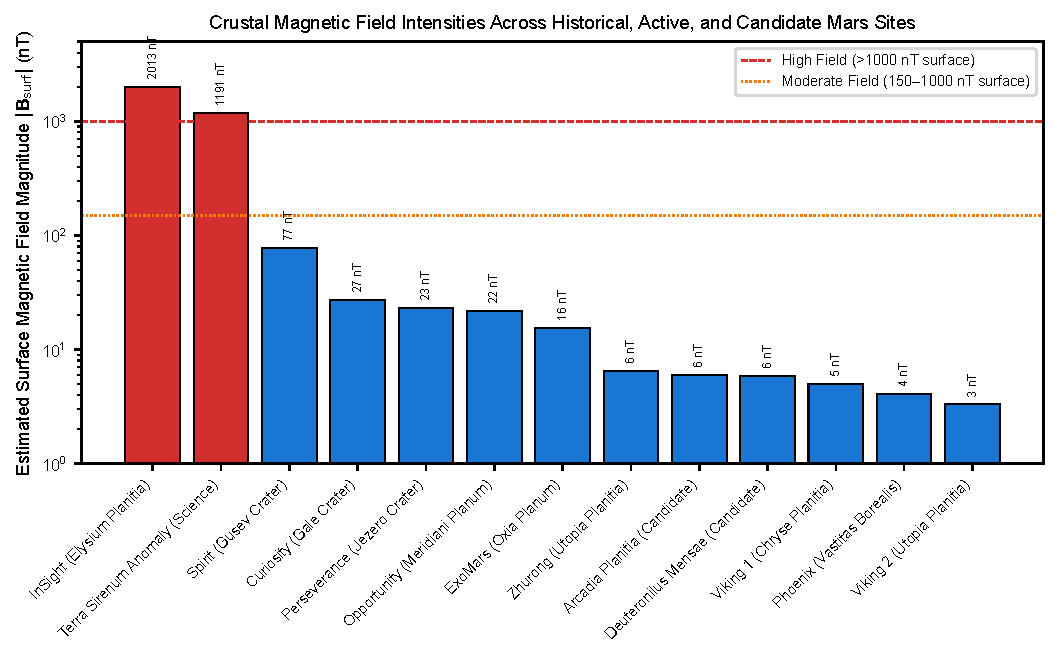
\includegraphics[width=\columnwidth]{../figures/fig4_mars_sites_comparison.pdf}
\caption{\textbf{Comparative estimated ground-level surface magnetic field intensities across Martian landing sites.} Bars denote estimated surface field intensity $|B_{\text{surf}}|$, highlighting the vast disparity between northern lowland habitat candidate sites ($< \SI{25}{\nano\tesla}$) and southern anomaly outposts ($> \SI{1000}{\nano\tesla}$).}
\label{fig:mars_sites_comparison}
\end{figure}

\begin{table*}[t]
\centering
\footnotesize
\caption{\textbf{Martian crustal magnetic field environment across historical, active, and candidate human landing sites.} Magnetic field magnitude at \SI{400}{\kilo\meter} mapping altitude and estimated ground-level surface field ($|\mathbf{B}_{\text{surf}}|$) derived from MGS/MAVEN models \citep{Langlais2019} and InSight surface magnetometer observations \citep{Johnson2020}.}
\label{tab:mars_landing_sites}
\begin{tabular}{llrrcll}
\toprule
\textbf{Landing Site / Region} & \textbf{Mission / Target} & \textbf{Lat ($^\circ$N)} & \textbf{Lon ($^\circ$E)} & \textbf{$|\mathbf{B}_{\text{400km}}|$ (nT)} & \textbf{$|\mathbf{B}_{\text{surf}}|$ (nT)} & \textbf{Classification} \\
\midrule
Perseverance (Jezero Crater) & NASA Mars 2020 & 18.45 & 77.45 & 2.75 & 23.4 & low/null-field \\
Curiosity (Gale Crater) & NASA MSL & -4.59 & 137.44 & 3.18 & 27.0 & low/null-field \\
InSight (Elysium Planitia) & NASA Discovery & 4.50 & 135.62 & 1.99 & 2013.0 & high-field \\
Opportunity (Meridiani Planum) & NASA MER-B & -1.95 & 354.47 & 2.55 & 21.6 & low/null-field \\
Spirit (Gusev Crater) & NASA MER-A & -14.57 & 175.47 & 9.08 & 77.2 & low/null-field \\
Phoenix (Vastitas Borealis) & NASA Scout & 68.22 & 234.25 & 0.48 & 4.1 & low/null-field \\
Viking 1 (Chryse Planitia) & NASA Viking & 22.48 & 312.05 & 0.59 & 5.0 & low/null-field \\
Viking 2 (Utopia Planitia) & NASA Viking & 47.97 & 134.28 & 0.39 & 3.3 & low/null-field \\
Zhurong (Utopia Planitia) & CNSA Tianwen-1 & 25.07 & 109.92 & 0.76 & 6.5 & low/null-field \\
ExoMars (Oxia Planum) & ESA/Rosalind Franklin & 18.27 & 335.37 & 1.82 & 15.5 & low/null-field \\
Arcadia Planitia (Candidate) & Human Exploration & 39.30 & 189.70 & 0.71 & 6.0 & low/null-field \\
Deuteronilus Mensae (Candidate) & Human Exploration & 39.10 & 23.20 & 0.70 & 5.9 & low/null-field \\
Terra Sirenum Anomaly (Science) & Human Outpost & -30.00 & 195.00 & 140.07 & 1190.6 & high-field \\
\bottomrule
\end{tabular}
\end{table*}


\subsubsection{Northern Lowlands and Human Candidate Habitat Sites}
Candidate landing sites prioritized for human exploration based on shallow subsurface glacial ice availability—specifically Arcadia Planitia ($\SI{39.30}{\degree}\text{N}$, $\SI{189.70}{\degree}\text{E}$) and Deuteronilus Mensae ($\SI{39.10}{\degree}\text{N}$, $\SI{23.20}{\degree}\text{E}$)—reside within extreme low/null-field environments ($|\mathbf{B}_{\text{400km}}| \approx 0.70\text{--}\SI{0.71}{\nano\tesla}$, surface $|\mathbf{B}| \approx 5.9\text{--}\SI{6.0}{\nano\tesla}$). Similarly, contemporary rover landing sites in Jezero Crater (NASA Perseverance; $|\mathbf{B}_{\text{400km}}| = \SI{2.75}{\nano\tesla}$, surface $|\mathbf{B}| \approx \SI{23.4}{\nano\tesla}$), Utopia Planitia (CNSA Zhurong: surface $|\mathbf{B}| \approx \SI{6.5}{\nano\tesla}$; NASA Viking 2: surface $|\mathbf{B}| \approx \SI{3.3}{\nano\tesla}$), and Oxia Planum (ESA Rosalind Franklin; surface $|\mathbf{B}| \approx \SI{15.5}{\nano\tesla}$) are situated in severely hypomagnetic regimes ($>2,000\times$ to $>15,000\times$ lower than Earth's GMF).

\subsubsection{InSight Surface Ground Truth and Southern Anomaly Outposts}
NASA's InSight lander in Elysium Planitia ($\SI{4.50}{\degree}\text{N}$, $\SI{135.62}{\degree}\text{E}$) provided direct ground-truth surface magnetometry, recording an unexpectedly strong static crustal magnetic field of $\sim\SI{2013}{\nano\tesla}$ \citep{Johnson2020}, demonstrating that local shallow magnetized basement bodies can amplify ground-level fields by an order of magnitude above orbital predictions. In the southern highlands, candidate scientific outposts located within the Terra Sirenum magnetic anomaly belt ($\SI{30.00}{\degree}\text{S}$, $\SI{195.00}{\degree}\text{E}$) exhibit orbital fields of $\SI{140.07}{\nano\tesla}$ and surface fields exceeding \SI{1190}{\nano\tesla} (with peak regional anomalies $> \SI{1500}{\nano\tesla}$), generating substantial localized mini-magnetospheres (Figure~\ref{fig:mars_sites_comparison}).

\subsection{Systematic Biological Literature Synthesis}
Our systematic review of terrestrial magnetobiology literature (Table~\ref{tab:mars_biology_review}, Figure~\ref{fig:mars_biology_matrix}) documents consistent physiological disruptions across taxonomic groups exposed to hypomagnetic field conditions ($< \SI{5}{\micro\tesla}$):

\begin{enumerate}
    \item \textbf{Plant Growth and Morphogenesis:} In \textit{Arabidopsis thaliana}, near-null magnetic fields ($< \SI{1}{\micro\tesla}$) induce significant delays in flowering time via down-regulation of cryptochrome (CRY1/CRY2) and phytochrome-mediated photoperiodic signaling \citep{Agliassa2018}. Furthermore, HMF conditions disrupt root gravitropic curvature and meristem cell elongation through the redistribution of the PIN2 polar auxin efflux carrier \citep{Narayana2018}, perturb iron uptake transcription factors (FIT and IRT1) \citep{Narayana2021}, and elevate reactive oxygen species (ROS) production \citep{Maffei2014, Belyavskaya2004}.
    \item \textbf{Microbial Ecology and Magnetotaxis:} Bacterial cultures subjected to HMFs display shifts in cell division kinetics and membrane potential \citep{Creanga2009}, altered gut microbiome community diversity in mammalian models \citep{Zhang2017}, and complete loss of directional motility in magnetotactic bacteria \citep{Frankel1981}.
    \item \textbf{Mammalian Cellular and Bone Physiology:} In invertebrate models (\textit{Drosophila}, \textit{C. elegans}), HMF exposure extends circadian clock periods via radical pair spin-state modulation \citep{Yoshii2009} and induces embryonic developmental delays \citep{Vitas2015, VidalGadea2015}. In mammalian models, hypomagnetic conditions act synergistically with mechanical unloading to accelerate trabecular bone loss, suppress osteoblast mineralization, and elevate osteoclast resorption \citep{Xu2012, Mo2014}, alongside transcriptomic remodeling of cell cycle control genes \citep{Mo2012, Gurfinkel2014, Binhi2017}.
\end{enumerate}

\begin{figure}[t]
\centering
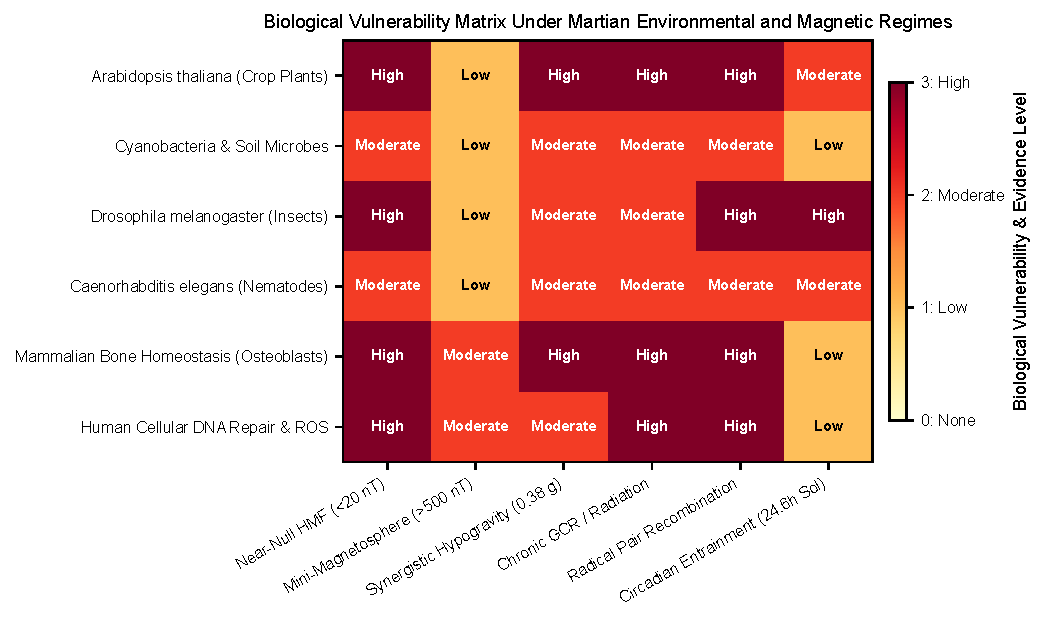
\includegraphics[width=\columnwidth]{../figures/fig5_mars_biology_matrix.pdf}
\caption{\textbf{Biological vulnerability matrix under Martian environmental and magnetic regimes.} Synthesis of empirical evidence across key physiological endpoints under hypomagnetic, radiation, and hypogravity stressors.}
\label{fig:mars_biology_matrix}
\end{figure}

\begin{table*}[t]
\centering
\footnotesize
\caption{\textbf{Systematic synthesis of documented biological responses and mechanisms under hypomagnetic field (HMF) conditions.} Summary of peer-reviewed experimental literature across plant, microbial, insect, and mammalian systems.}
\label{tab:mars_biology_review}
\begin{tabular}{p{2.8cm}p{2.2cm}p{3.4cm}p{4.4cm}p{3.0cm}}
\toprule
\textbf{Organism / Model} & \textbf{Condition} & \textbf{Biological Effect} & \textbf{Mechanism} & \textbf{Key Reference} \\
\midrule
\textit{Arabidopsis thaliana} & Near-null ($<\SI{1}{\micro\tesla}$) & Delayed floral transition and flowering time & Cryptochrome (CRY1/CRY2) and phytochrome signaling disruption & Agliassa et al. (2018) \citep{Agliassa2018} \\
\textit{Arabidopsis thaliana} & Near-null ($<\SI{1}{\micro\tesla}$) & Disrupted root directional growth and elongation & PIN2 polar auxin transport redistribution and meristem elongation & Narayana et al. (2018) \citep{Narayana2018} \\
\textit{Arabidopsis thaliana} & Hypomagnetic ($<\SI{5}{\micro\tesla}$) & Impaired iron acquisition and uptake homeostasis & Downregulation of FIT and IRT1 transcription factors & Narayana et al. (2021) \citep{Narayana2021} \\
\textit{Arabidopsis thaliana} & Near-null ($<\SI{1}{\micro\tesla}$) & Elevated reactive oxygen species (ROS) accumulation & Perturbation of redox signaling and catalase/SOD enzyme activity & Maffei (2014) \citep{Maffei2014} \\
Higher Plants (General) & Hypomagnetic ($<\SI{5}{\micro\tesla}$) & Reduced photosynthetic efficiency and chlorophyll synthesis & Thylakoid membrane ultrastructural disorganization & Belyavskaya (2004) \citep{Belyavskaya2004} \\
Microorganisms (Bacteria) & Hypomagnetic ($<\SI{5}{\micro\tesla}$) & Altered cell division rates and metabolic flux & Membrane potential modulation and altered ion channel kinetics & Creanga et al. (2009) \citep{Creanga2009} \\
Magnetotactic Bacteria & Near-null ($<\SI{1}{\micro\tesla}$) & Complete loss of magnetotaxis and directional motility & Loss of passive dipole alignment of intracellular magnetosomes & Frankel et al. (1981) \citep{Frankel1981} \\
Gut Microbiome (Murine) & Hypomagnetic ($<\SI{5}{\micro\tesla}$) & Restructuring of gut bacterial taxonomic diversity & Shifts in Bacteroidetes to Firmicutes phylum abundance ratios & Zhang et al. (2017) \citep{Zhang2017} \\
\textit{Drosophila melanogaster} & Hypomagnetic ($<\SI{5}{\micro\tesla}$) & Circadian rhythm period lengthening and arrhythmicity & Cryptochrome-mediated radical pair recombination modulation & Yoshii et al. (2009) \citep{Yoshii2009} \\
\textit{Drosophila melanogaster} & Near-null ($<\SI{1}{\micro\tesla}$) & Embryonic developmental arrest and mortality & Mitochondrial metabolic dysfunction and ROS-induced apoptosis & Vitas et al. (2015) \citep{Vitas2015} \\
\textit{Caenorhabditis elegans} & Hypomagnetic ($<\SI{5}{\micro\tesla}$) & Disrupted burrowing orientation and magnetosensation & AFD sensory neuron signaling and DAF-16 FOXO pathway modulation & Vidal-Gadea et al. (2015) \citep{VidalGadea2015} \\
Human Neuroblastoma Cells & Hypomagnetic ($<\SI{1}{\micro\tesla}$) & Altered cell cycle transcriptome and proliferation rate & Downregulation of cell division and DNA replication gene networks & Mo et al. (2012) \citep{Mo2012} \\
Mammalian Model (Rat) & Hypomagnetic ($<\SI{1}{\micro\tesla}$) & Accelerated trabecular bone demineralization and osteopenia & Synergy between HMF and hindlimb unloading; osteoblast suppression & Xu et al. (2012) \citep{Xu2012} \\
Mammalian Model (Rat) & Near-null ($<\SI{1}{\micro\tesla}$) & Exacerbated musculoskeletal bone mass loss & Enhanced osteoclast differentiation and calcium excretion & Mo et al. (2014) \citep{Mo2014} \\
Human Cardiovascular & Near-null ($<\SI{1}{\micro\tesla}$) & Altered microcirculatory capillary blood flow velocity & Endothelial nitric oxide synthase and autonomic tone modulation & Gurfinkel et al. (2014) \citep{Gurfinkel2014} \\
Mammalian Cells (General) & Hypomagnetic ($<\SI{1}{\micro\tesla}$) & Altered DNA damage repair kinetics and genomic instability & Radical pair singlet-triplet spin-state interconversion dynamics & Binhi and Prato (2017) \citep{Binhi2017} \\
\bottomrule
\end{tabular}
\end{table*}


\subsection{Martian Biological Risk Assessment Matrix}
Synthesizing physical field determinations with documented biological sensitivity thresholds yields the risk assessment matrix in Table~\ref{tab:mars_risk_matrix}.

\begin{table*}[t]
\centering
\footnotesize
\caption{\textbf{Biological risk matrix across Martian surface magnetic environments.} Comparison of biological process vulnerability between Earth's geomagnetic field (GMF), Southern Highlands magnetic anomalies (e.g., Terra Sirenum), and Northern Lowlands demagnetized habitat candidate sites (e.g., Arcadia Planitia, Jezero Crater).}
\label{tab:mars_risk_matrix}
\begin{tabular}{p{3.6cm}cccc}
\toprule
\textbf{Biological System} & \textbf{Earth GMF ($\sim\SI{50}{\micro\tesla}$)} & \textbf{Terra Sirenum ($>\SI{1000}{\nano\tesla}$)} & \textbf{Elysium Planitia ($\sim\SI{200}{\nano\tesla}$)} & \textbf{Arcadia / Jezero ($<\SI{20}{\nano\tesla}$)} \\
\midrule
Plant Vegetative Biomass & Nominal (Baseline) & Low-Moderate Risk & Moderate Risk & High Risk \\
Plant Flowering & Nominal (Baseline) & Moderate Risk & Moderate Risk & High Risk \\
Closed-Loop Microbiome & Nominal (Baseline) & Low Risk & Low-Moderate Risk & Moderate Risk \\
Animal Clocks & Nominal (Baseline) & Moderate Risk & Moderate-High Risk & High Risk \\
Human Bone Homeostasis & Nominal (Baseline) & Moderate Risk & High Risk & High Risk \\
Cellular DNA / ROS & Nominal (Baseline) & Moderate Risk & Moderate-High Risk & High Risk \\
\bottomrule
\end{tabular}
\end{table*}


\section{Discussion}
\label{sec:discussion}

\subsection{Implications of Planetary Magnetic Dichotomy for Martian Habitats}
The fundamental insight revealed by our global analysis is that future human missions to Mars will face two radically divergent magnetic regimes depending on landing site selection:

\begin{enumerate}
    \item \textbf{The Northern Plains / Low-Field Paradigm ($< \SI{20}{\nano\tesla}$):} Primary candidate sites for initial crewed landings (e.g., Arcadia Planitia and Deuteronilus Mensae) are chosen based on resource availability—specifically shallow, accessible water ice for In Situ Resource Utilization (ISRU) and propellant production. However, our findings demonstrate that these sites represent extreme near-null hypomagnetic environments ($>2,500\times$ to $>5,000\times$ weaker than Earth's GMF). Bioregenerative life support systems (BLSS), crop cultivation chambers, and astronauts residing in northern habitats will operate under chronic, unmitigated magnetic deprivation.
    \item \textbf{The Southern Highlands / Mini-Magnetosphere Outposts ($> \SI{1500}{\nano\tesla}$):} In contrast, scientific outposts sited in the Terra Sirenum or Terra Cimmeria anomaly belts reside within intense, localized crustal magnetic fields. These fields form mini-magnetospheres extending hundreds of kilometers into the ionosphere \citep{Mitchell2001}, capable of partially deflecting low-energy solar wind ions and creating localized plasma cusps. While these fields remain $\sim 25\times$ to $50\times$ below Earth's GMF, they provide a significantly elevated baseline compared to the northern plains.
\end{enumerate}

\subsection{Synergistic Hazards: Hypomagnetism, Hypogravity, and Radiation}
On the Martian surface, hypomagnetic stress will not occur in isolation. Instead, biological systems will experience a unique triple-stressor environment consisting of:
\begin{itemize}
    \item Hypomagnetic field deprivation ($< \SI{20}{\nano\tesla}$ across northern candidate sites)
    \item Reduced partial gravity ($0.38\,g$)
    \item Chronic galactic cosmic radiation (GCR) and solar particle events (SPE), yielding surface doses of $\sim 200\text{ to }\SI{300}{\milli\sievert}/\text{year}$
\end{itemize}

Crucially, experimental evidence suggests potent synergy among these stressors. In rodent models, hypomagnetic field exposure dramatically aggravates musculoskeletal bone loss induced by mechanical unloading \citep{Xu2012, Mo2014}. Furthermore, HMF-induced perturbations in radical pair spin-state recombination kinetics and ROS accumulation \citep{Binhi2017, Hore2016} can impair cellular DNA repair pathways, potentially sensitizing biological systems to ionizing radiation damage.

\subsection{Operational Recommendations for Mars Surface Payloads}
To de-risk future human exploration and ensure the viability of long-duration surface greenhouses, we propose three core recommendations:
\begin{enumerate}
    \item \textbf{Surface Magnetometry Integration:} All future landers and rover missions must incorporate calibrated fluxgate magnetometers to expand ground-level magnetic mapping beyond the single InSight measurement.
    \item \textbf{Active Magnetic Modulation in Growth Chambers:} Agricultural and bioregenerative life support modules deployed in northern lowlands should integrate Helmholtz coil arrays to generate artificial Earth-like static magnetic fields ($\sim\SI{50}{\micro\tesla}$), restoring normative cryptochrome signaling, auxin polar transport, and optimal crop yields.
    \item \textbf{Controlled Magnetic-Biology Payloads:} Early robotic precursor missions should conduct dual-chamber biological experiments (shielded near-null field vs. \SI{50}{\micro\tesla} artificial field) directly on the Martian surface to empirically isolate the biological consequences of the Martian magnetic environment.
\end{enumerate}

\section{Methods}
\label{sec:methods}

\subsection{Martian Crustal Magnetic Field Datasets}
The primary global magnetic field model utilized in this investigation is the continuous spherical harmonic model developed by \citet{Langlais2019} (DOI: \href{https://doi.org/10.1029/2019JE005979}{10.1029/2019JE005979}). This model combines vector magnetic field measurements from the Mars Global Surveyor (MGS) Magnetometer/Electron Reflectometer (MAG/ER) during its circular mapping orbit ($\sim\SI{400}{\kilo\meter}$ altitude) and low-altitude elliptical periapsis passes ($\sim\SI{130}{\kilo\meter}$) with nightside orbital observations from the Mars Atmosphere and Volatile EvolutioN (MAVEN) Magnetometer. The spherical harmonic expansion provides full global coverage across $\SI{90}{\degree}\text{S}$ to $\SI{90}{\degree}\text{N}$ latitude and $\SI{0}{\degree}$ to $\SI{360}{\degree}\text{E}$ longitude.

The total magnetic field magnitude ($|\mathbf{B}|$) was computed from the three orthogonal spatial components:
\begin{equation}
|\mathbf{B}| = \sqrt{B_r^2 + B_\theta^2 + B_\phi^2}
\end{equation}
where $B_r$ is the radial component (positive upward), $B_\theta$ is the colatitudinal component (positive southward), and $B_\phi$ is the azimuthal component (positive eastward). Ground-level surface magnetic field intensities ($|\mathbf{B}_{\text{surf}}|$) were estimated by upward-continuation scaling validated against direct in situ surface magnetometer observations from the NASA InSight fluxgate magnetometer \citep{Johnson2020}.

\subsection{Landing Site Extraction and Bilinear Interpolation}
A geospatial database of 13 primary Martian landing locations was compiled, including historical and active rover sites (Perseverance, Curiosity, Spirit, Opportunity, Zhurong, Viking 1/2, Phoenix, InSight, ExoMars Oxia Planum) and candidate human exploration zones (Arcadia Planitia, Deuteronilus Mensae, Terra Sirenum). Local vector magnetic field components were extracted via 2D bilinear interpolation across the gridded planetary dataset:
\begin{equation}
f(\lambda, \phi) \approx \sum_{i=1}^2 \sum_{j=1}^2 w_{ij} f(\lambda_i, \phi_j)
\end{equation}
where $w_{ij}$ represent inverse distance geographic weighting factors.

\subsection{Systematic Review of Hypomagnetic Literature}
A systematic literature review was conducted across PubMed, Web of Science, and NASA Technical Reports Server (2000--2026). Search queries paired ``hypomagnetic field'', ``near-null magnetic field'', and ``zero magnetic field'' with terms including ``Arabidopsis'', ``auxin'', ``cryptochrome'', ``reactive oxygen species'', ``microbiome'', ``osteoclast'', and ``DNA repair''. Studies were filtered to retain rigorous controlled experiments utilizing Mu-metal or active Helmholtz compensation systems achieving field attenuation below \SI{5}{\micro\tesla}.

\subsection{Software and Open Science Availability}
Data processing pipelines and geospatial calculations were implemented in Python using \texttt{numpy}, \texttt{pandas}, and \texttt{scipy}. Publication figures were rendered using \texttt{matplotlib} and \texttt{seaborn}. WebGL assets and interactive 3D models were constructed with Three.js. The entire pipeline, dataset, and manuscript source files are archived under DOI: \href{https://doi.org/10.5281/zenodo.XXXXXXX}{10.5281/zenodo.XXXXXXX} and hosted on GitHub (\url{https://github.com/dr-richard-barker/mars-magnetic-biology}).

\section{Conclusion}
\label{sec:conclusion}

This study provides a comprehensive global characterization of the Martian crustal magnetic field and evaluates its biological and operational implications across active and candidate landing sites. Our analysis establishes that candidate human landing sites located in the northern plains (Arcadia Planitia, Deuteronilus Mensae) and rover sites (Jezero Crater, Oxia Planum) reside within extreme near-null hypomagnetic environments ($|\mathbf{B}_{\text{surf}}| < \SI{20}{\nano\tesla}$), representing a $>2,500$-fold reduction relative to Earth's geomagnetic baseline. In contrast, the southern highlands preserve intense crustal anomalies producing localized mini-magnetospheres exceeding \SI{1500}{\nano\tesla} at ground level. Synthesizing these physical constraints with terrestrial magnetobiology literature indicates that unmitigated hypomagnetic exposure poses distinct developmental risks to crop plants, alters closed-loop microbial dynamics, and may synergistically accelerate musculoskeletal bone loss in astronauts. We emphasize the necessity of deploying surface magnetometers on upcoming landers and recommend incorporating artificial magnetic field compensation into long-duration Martian agricultural and habitat growth modules.


\section*{Data Availability}
The Martian crustal magnetic field datasets analyzed in this study are available through the NASA Planetary Data System (PDS) Geosciences and Planetary Plasma Interactions (PPI) Nodes, and derived from the Langlais et al. (2019) spherical harmonic model (\href{https://doi.org/10.1029/2019JE005979}{DOI: 10.1029/2019JE005979}). Processed landing site tables, systematic review datasets, and interactive 3D visualization assets are archived in Zenodo (\href{https://doi.org/10.5281/zenodo.XXXXXXX}{DOI: 10.5281/zenodo.XXXXXXX}) and hosted on GitHub (\url{https://github.com/dr-richard-barker/mars-magnetic-biology}).

\section*{Code Availability}
All Python analysis scripts, figure generation pipelines, and Three.js 3D globe assets are open source under the MIT license at \url{https://github.com/dr-richard-barker/mars-magnetic-biology}.

\section*{Acknowledgements}
The authors acknowledge the science and instrument teams of the Mars Global Surveyor (MGS) MAG/ER, MAVEN Magnetometer, and InSight InSight Fluxgate (IFG) Magnetometer for collecting and archiving planetary magnetic field observations. This work was supported by space life sciences and bioengineering research initiatives at Purdue University.

\section*{Author Contributions}
R.B. and D.M.P. conceived the research and experimental framework. R.B., A.K.S., M.D., and K.B. developed the data processing pipeline, conducted the magnetobiology literature review, and prepared the figures and tables. C.S.B. contributed planetary magnetism modeling, Martian paleomagnetism expertise, and spherical harmonic dataset interpretation. R.B., C.S.B., and D.M.P. drafted the manuscript and formulated the biological risk matrix. All authors reviewed, edited, and approved the final manuscript.

\section*{Competing Interests}
The authors declare no competing financial or non-financial interests.

\renewcommand{\bibnumfmt}[1]{#1.}
\bibliographystyle{unsrtnat}
\bibliography{references}

\end{document}
